%\documentclass[12pt, letterpaper]{article} 
% report: Estilo Informe completo, con capítulos.
% article: Estilo Informe básico, sin Capítulos.

\usepackage[T1]{fontenc}
\usepackage[utf8x]{inputenc}
\usepackage[activeacute,spanish,es-tabla]{babel} % Idioma español, con sus configuraciones
\usepackage[left=2cm, right=2cm, bottom=3cm, top=3cm, headheight=40pt]{geometry} % Márgenes
\usepackage{graphicx} % Required for including pictures
\usepackage{float} % Allows putting an [H] in \begin{figure} to specify the exact location of the figure
\usepackage{wrapfig} % Allows in-line images
\usepackage[nottoc, notlot, notlof]{tocbibind} % Índices, sin ToC, LoF ni LoT
\renewcommand{\refname}{Bibliografía} % Nombre para Bibliografía (clase article)
%\renewcommand{\bibname}{Bibliografía} % Nombre para Bibliografía (clase book/report)
\renewcommand\tocbibname{Bibliografía}
\usepackage{amsmath}
\usepackage{amsfonts}
\usepackage{amssymb}
\usepackage{siunitx} % Unidades del SI
\sisetup{output-decimal-marker = {,}}
\usepackage{cancel} % Permite cancelar (tachar) elementos
\usepackage{tabu} % Tablas chéveres
\usepackage{booktabs} % Allows the use of \toprule, \midrule and \bottomrule in tables for horizontal lines
\usepackage{multirow} % Celdas en más de una fila
\usepackage{multicol}
\usepackage{easybmat} % Matrices por Bloques
\usepackage{lipsum} % Lorem Ipsum


\usepackage{color}
\definecolor{gray51}{rgb}{0.51,0.51,0.51}
\definecolor{gray71}{rgb}{0.71,0.71,0.71}
\newcommand{\HRule}{\rule{\linewidth}{.4mm}}

\usepackage{listings} % Incluye códigos
\renewcommand{\lstlistingname}{Algoritmo}
\renewcommand{\lstlistlistingname}{Índice de \lstlistingname s}
\lstset{ 
	basicstyle=\ttfamily\small,
    commentstyle=\color{red},
    keywordstyle=\color{blue},
    numberstyle=\tiny\color{gray71},
    stringstyle=\color{green},
    breakatwhitespace=false,         
    breaklines=true,                 
    captionpos=b,                    
    keepspaces=true,                 
    numbers=left,                    
    numbersep=5pt,                  
    showspaces=false,                
    showstringspaces=false,
    showtabs=false,                  
    tabsize=2,
    xleftmargin=2em,
    frame=single,
    framexleftmargin=1.5em
}

\usepackage{hyperref} 		% Hipervínculos
\hypersetup{
	colorlinks	= true,		% Vínculos coloreados en vez de recuadros
    urlcolor	= blue,		% Color para vínculos externos
    linkcolor	= black,	% Color para vínculos internos
    citecolor	= red		% Color para citas
}
\documentclass[12pt, letterpaper]{article} 
% report: Estilo Informe completo, con capítulos.
% article: Estilo Informe básico, sin Capítulos.

\usepackage[T1]{fontenc}
\usepackage[utf8x]{inputenc}
\usepackage[activeacute,spanish,es-nodecimaldot,es-tabla]{babel} % Idioma español, con sus configuraciones
\usepackage[left=2cm, right=2cm, bottom=3cm, top=3cm, headheight=40pt]{geometry} % Márgenes
\usepackage{graphicx} % Required for including pictures
\usepackage{float} % Allows putting an [H] in \begin{figure} to specify the exact location of the figure
\usepackage{wrapfig} % Allows in-line images
\usepackage[nottoc, notlot, notlof]{tocbibind} % Índices, sin ToC, LoF ni LoT
\renewcommand{\refname}{Bibliografía} % Nombre para Bibliografía (clase article)
%\renewcommand{\bibname}{Bibliografía} % Nombre para Bibliografía (clase book/report)
\renewcommand\tocbibname{Bibliografía}
\usepackage{amsmath}
\usepackage{amsfonts}
\usepackage{amssymb}
%\usepackage{siunitx} % Unidades del SI
%\sisetup{output-decimal-marker = {.}}
\usepackage{cancel} % Permite cancelar (tachar) elementos
\usepackage{tabu} % Tablas chéveres
\usepackage{booktabs} % Allows the use of \toprule, \midrule and \bottomrule in tables for horizontal lines
\usepackage{multirow} % Celdas en más de una fila
\usepackage{multicol}
\usepackage{easybmat} % Matrices por Bloques
\usepackage{lipsum} % Lorem Ipsum


\usepackage{color}
\definecolor{gray51}{rgb}{0.51,0.51,0.51}
\definecolor{gray71}{rgb}{0.71,0.71,0.71}
\newcommand{\HRule}{\rule{\linewidth}{.4mm}}

\usepackage{listings} % Incluye códigos
\renewcommand{\lstlistingname}{Algoritmo}
\renewcommand{\lstlistlistingname}{Índice de \lstlistingname s}
\lstset{ 
	basicstyle=\ttfamily\small,
    commentstyle=\color{red},
    keywordstyle=\color{blue},
    numberstyle=\tiny\color{gray71},
    stringstyle=\color{green},
    breakatwhitespace=false,         
    breaklines=true,                 
    captionpos=b,                    
    keepspaces=true,                 
    numbers=left,                    
    numbersep=5pt,                  
    showspaces=false,                
    showstringspaces=false,
    showtabs=false,                  
    tabsize=2,
    xleftmargin=2em,
    frame=single,
    framexleftmargin=1.5em
}

\usepackage{hyperref} 		% Hipervínculos
\hypersetup{
	colorlinks	= true,		% Vínculos coloreados en vez de recuadros
    urlcolor	= blue,		% Color para vínculos externos
    linkcolor	= black,	% Color para vínculos internos
    citecolor	= red		% Color para citas
}

\title{Informe tarea 1} % Nombre archivo en Overleaf
\newcommand{\ramo}{EL7008-1 Procesamiento Avanzado de Imágenes}
\newcommand{\departamento}{Departamento de Ingeniería Eléctrica}
\newcommand{\semestre}{Semestre Primavera 2020}

\newcommand{\hipertitulo}{}
\newcommand{\titulo}{Tarea 1} 
\newcommand{\subtitulo}{Piramides de \textit{Gauss} y \textit{Laplace}}

\newcommand{\autor}{Diego Irarrázaval I.}


\usepackage{fancyhdr}
\pagestyle{fancy}
\fancyhead[L]{\footnotesize Universidad de Chile - Facultad de Ciencias Físicas y Matemáticas\\
\departamento\\
\ramo\ - \semestre}
\fancyhead[R]{
\includegraphics[scale=0.2]{fcfm.png}}
\fancyfoot[L]{\small \rm \textit{\titulo}}
\fancyfoot[C]{}
\fancyfoot[R]{\small \rm \textbf{\thepage}}
\renewcommand{\headrulewidth}{0.5pt}
\renewcommand{\footrulewidth}{0.5pt}
\renewcommand{\lstlistingname}{Código}
\renewcommand{\lstlistlistingname}{Índice de \lstlistingname s}
\lstdefinestyle{style_def}{ 
	basicstyle=\ttfamily\small,
    commentstyle=\color{red},
    keywordstyle=\color{blue},
    numberstyle=\tiny\color{gray71},
    stringstyle=\color{green},
    breakatwhitespace=false,         
    breaklines=true,                 
    captionpos=b,                    
    keepspaces=true,                 
    numbers=left,                    
    numbersep=5pt,                  
    showspaces=false,                
    showstringspaces=false,
    showtabs=false,                  
    tabsize=2,
    xleftmargin=2em,
    frame=single,
    framexleftmargin=1.5em
}

\definecolor{codegreen}{rgb}{0,0.6,0}
\definecolor{codegray}{rgb}{0.5,0.5,0.5}
\definecolor{codepurple}{rgb}{0.58,0,0.82}
\definecolor{backcolour}{rgb}{0.95,0.95,0.92}
 
\lstdefinestyle{mystyle}{
    backgroundcolor=\color{backcolour},   
    commentstyle=\color{codegreen},
    keywordstyle=\color{magenta},
    numberstyle=\tiny\color{codegray},
    stringstyle=\color{codepurple},
    basicstyle=\ttfamily\footnotesize,
    breakatwhitespace=false,         
    breaklines=true,                 
    captionpos=b,                    
    keepspaces=true,                 
    numbers=left,                    
    numbersep=5pt,                  
    showspaces=false,                
    showstringspaces=false,
    showtabs=false,                  
    tabsize=2
}

\lstset{style=mystyle}
% Default fixed font does not support bold face
\DeclareFixedFont{\ttb}{T1}{txtt}{bx}{n}{12} % for bold
\DeclareFixedFont{\ttm}{T1}{txtt}{m}{n}{12}  % for normal

% Custom colors
\usepackage{color}
\definecolor{deepblue}{rgb}{0,0,0.5}
\definecolor{deepred}{rgb}{0.6,0,0}
\definecolor{deepgreen}{rgb}{0,0.5,0}

\usepackage{listings}

% Python style for highlighting
\newcommand\pythonstyle{\lstset{
language=Python,
basicstyle=\ttm,
otherkeywords={self},             % Add keywords here
keywordstyle=\ttb\color{deepblue},
emph={MyClass,__init__},          % Custom highlighting
emphstyle=\ttb\color{deepred},    % Custom highlighting style
stringstyle=\color{deepgreen},
frame=tb,                         % Any extra options here
showstringspaces=false            % 
}}


% Python environment
\lstnewenvironment{python}[1][]
{
\pythonstyle
\lstset{#1}
}
{}

% Python for external files
\newcommand\pythonexternal[2][]{{
\pythonstyle
\lstinputlisting[#1]{#2}}}

% Python for inline
\newcommand\pythoninline[1]{{\pythonstyle\lstinline!#1!}}

%\linespread{1.2} 				% Interlineado
%\setlength\parindent{0pt} 		% Longitud sangría
\usepackage{subcaption}
\begin{document}
%----------------------------------------------------------------------
%	Portada
%----------------------------------------------------------------------
\newgeometry{left=2.5cm,right=2.5cm, top=2.5cm, bottom=2.5cm}

\begin{titlepage}
{
\begin{wrapfigure}{l}{1cm}
\vspace{-0.7cm}

\includegraphics[width=5cm]{fcfm.png}
\end{wrapfigure}

\textsc{\color{red}\hspace{3.2cm}\departamento}\\
\textsc{\color{gray51}\hspace{3.8cm}Facultad de Ciencias Físicas y Matemáticas}\\
\textsc{\color{gray51}\hspace{3.8cm}Universidad de Chile}\\
\textsc{\color{gray51}\hspace{3.8cm}\ramo}\\
}

\begin{center}
~\\[5cm]
{\color{gray71}\textsc{\hipertitulo}}
\HRule~ \\[0.4cm]
{ \Huge \textup \bfseries  \titulo}\\[0.4cm]
{ \Large \textup{\subtitulo}}\\[0.2cm]
\HRule \\ [0.4cm]
{ \Huge \textup \bfseries  \autor}\\
~\\[3.5cm]
\end{center}

\begin{minipage}{.5\textwidth}
~
\end{minipage}
\begin{minipage}{.45\textwidth}
\begin{flushright}
\begin{tabular}{l}
\textbf{\textit{Profesor:}} \\
{\small Javier Ruiz del Solar.}\\[0.3cm]

\textbf{\textit{Auxiliar:}} \\
{\small Patricio Loncomilla Z.}\\[0.3cm]

%\textbf{\textit{Integrantes:}}\\
%{\small Javier Rojas J.}\\[.3cm]

\textbf{\textit{Fecha:}}\\
{\small \today}
\end{tabular}
\end{flushright}
\end{minipage}
\begin{minipage}{.05\textwidth}
~
\end{minipage}
\end{titlepage}

\restoregeometry
%----------------------------------------------------------------------
%	Documento
%----------------------------------------------------------------------

\pagenumbering{Roman}
\setcounter{page}{1}
\tableofcontents 
\newpage
\listoffigures
\listoftables
\lstlistoflistings

%\addcontentsline{toc}{chapter}{Nombre Sección} % Para forzar aparición en el Índice

\newpage
\pagenumbering{arabic}
\setcounter{page}{1}

\newpage
\section{Introducción}

% \par Describir brevemente lo que se realizará en la tarea
\par En esta tarea, se implementará el cálculo de pirámides de \textit{Gauss} y \textit{Laplace} de una imagen y, luego, se reconstruirán a partir de dichas pirámides. Para lograr esto, se deberá implementar también la convolución en dos dimensiones. 
\par Los principales objetivos corresponden en primer lugar a introducir algunas formas de representaciones multi-resolución calculadas a partir de una images e implementar operaciones desde cero (por ejemplo la convolución) que usualmente se cargan con librerías. 

% \par Enumeración y explicación de las secciones que siguen
\bigskip

\par El informe comienza con el marco teórico donde se expone brevemente sobre la convolución, la pirámide de Gauss, la pirámide de Laplace y la reconstrucción de la imagen. 

\par A continuación, la sección desarrollo se divide en tres sub-secciones:
\begin{enumerate}
  \item Pirámide de Gauss.
  \item Pirámide de Laplace.
  \item Reconstrucción imagen. 
\end{enumerate}

\par En las secciones enumeradas anteriormente, se incluye tanto el código implementado como análisis teórico de lo desarrollado. 

\par Finalmente, se presentan las conclusiones del desarrollo de la tarea 1. 

\newpage
\section{Marco Teórico}
\subsection{Convolución}

\par En matemáticas, la convolución es una operación que recibe dos funciones ($f$ y $g$) y entrega una tercera función ($f \: \ast \: g $) que describe como la forma de una es influida por la otra \cite{WikiConv}.
\par En procesamiento de señales, se puede entender como afecta se ve afectada señal  pasar por un filtro. En este caso, la señal corresponde a una imagen y el filtro será otra imagen (le llamaremos indistintamente \textit{kernel}, \textit{mask} o máscara). A continuación, se muestra una ilustración que se utilizará para explicar la operación convolución en dos dimensiones:

\begin{figure}[H]
  \centering
  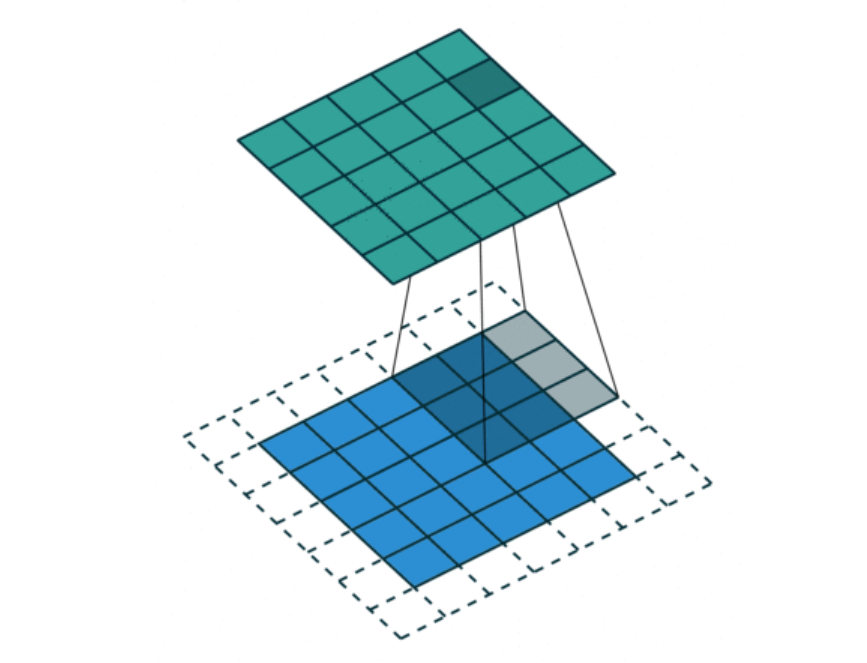
\includegraphics[width = 0.5\textwidth]{conv2d.png}
  \caption{Convolucion en dos dimensiones con padding.\cite{imConv2d}}
  \label{fig:conv2d}
\end{figure}

\par En la figura \ref{fig:conv2d} se observa una imagen de entrada (representada por la matriz de cuadrados azules) con 5 pixeles de ancho por 5 de largo. Adicionalmente, se agrega un pixel de ancho y uno de largo de color blanco. Éstos representan el \textit{padding}.El kernel por otro lado, se representa por los pixeles sombreados (kernel de 3x3).

\par Para el cálculo de la imagen de salida, se utiliza la siguiente ecuación:

\begin{align}
  y[i,j] = \sum_{m}^{M} \sum_{n}^{N} x[i-m, j-n] \cdot h[m,n] \: \: \: \: \forall i \in [0,Height], \: j \in [0,Width]
  \label{eqn:conv2d}
\end{align}

\par En la ecuación \ref{eqn:conv2d}, la imagen de salida (y), se construye con la operación del kernel (h) sobre todos los pixeles de la imagen de entrada (x) y los vecinos correspondientes.

\par En el ejemplo de la figura \ref{fig:conv2d}, se realiza \textit{padding}. Esto consiste en agrandar la imagen de entrada para que la salida sea de la misma dimension. En esta ocasión, se realizará padding con ceros, es decir, se rellenará con ceros donde sea necesario.

\subsection{Pirámides}
\par Como se menciono anteriormente, las pirámides corresponden a representaciones multi\-resolución calculadas a partir de imágenes. En éstas, la señal o imagen de entrada es filtrada y submuestreada tantas veces como niveles se quieran.


\par Inicialmente, las pirámides se utilizaron para la detección e identificación de objetos que pueden o no aparecer a distintas escalas. La idea, es crear distintas copias del objeto cambiando el tamaño (o escala) y resolución de estos. En la figura \ref{fig:pyramidPaper} se observan distintas resoluciones del mismo objeto para obtener otras representaciones.

\begin{figure}[H]
  \centering
  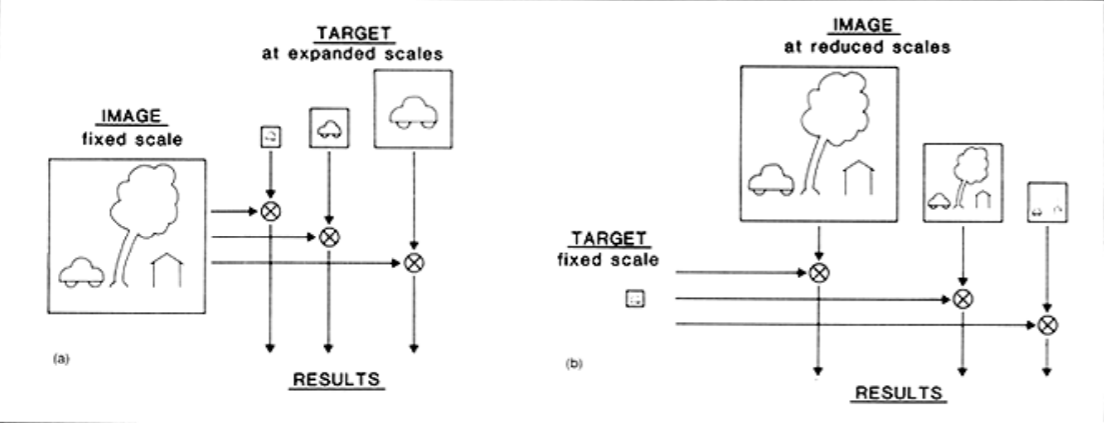
\includegraphics[width = 0.7\textwidth]{pyramid_paper.png}
  \caption{Distintas formas de utilizar las pirámides. En (a), copias del objeto a detectar se escalan. En (b), la imagen se trabaja completa. \cite{paperPyramids}}
  \label{fig:pyramidPaper}
\end{figure}


\subsubsection{Piramide de Gauss}
La pirámide de gauss corresponde a un caso particular de las pirámides en las que el filtro aplicado es uno pasabajo, con semejanzas a un filtro con distribución \textit{gaussiana}. 

\par En estos, se aplica un filtro \textit{gaussiano} a cada imagen y luego se sub-muestrea. El filtro  \textit{gaussiano} también se conoce como \textit{blur} y recibe como parámetro la desviación estándar a partir de la cual se originará el filtro. En la siguiente figura, se observa el efecto de variar la desviación estándar usada para el cálculo del filtro:

\begin{figure}[H]
  \centering
  \begin{subfigure}[t]{0.32\textwidth}
    \centering
    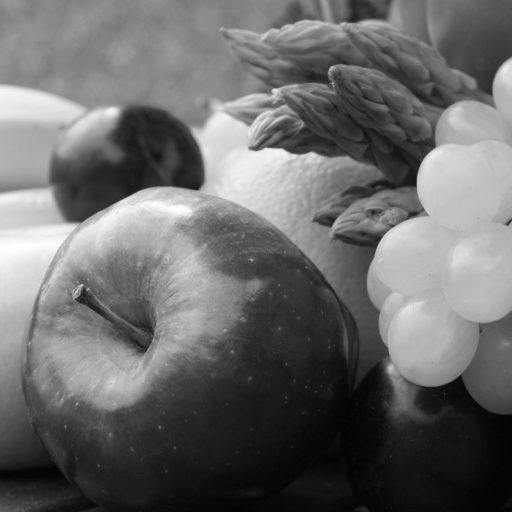
\includegraphics[width = 0.9\textwidth]{frutas.png}
    \caption{Imagen original (en blanco y negro).}
  \end{subfigure}
  ~
  \begin{subfigure}[t]{0.32\textwidth}
      \centering
      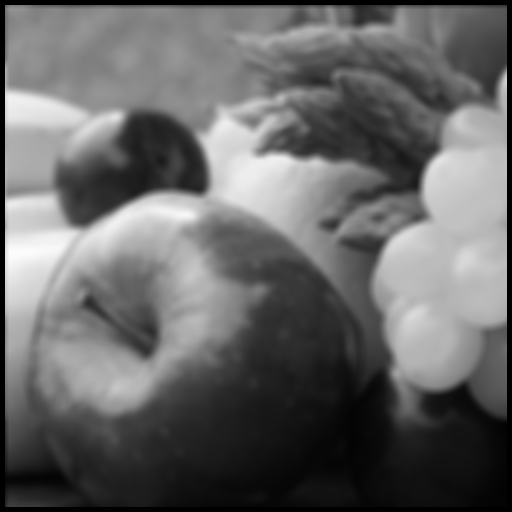
\includegraphics[width = 0.9\textwidth]{frutas_std5.png}
      \caption{Imagen con filtro \textit{blur} aplicado con $\sigma=5$.}
  \end{subfigure}
  ~ 
  \begin{subfigure}[t]{0.32\textwidth}
      \centering
      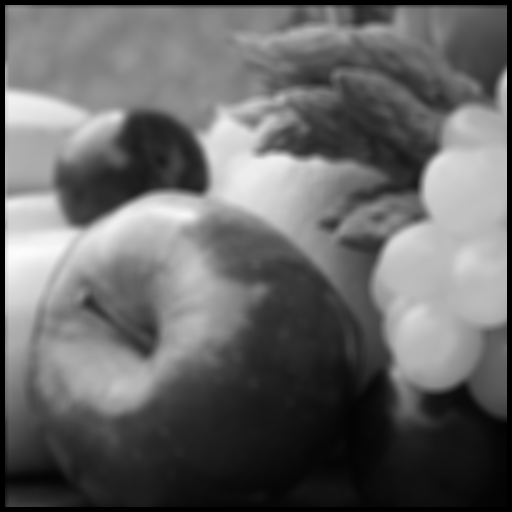
\includegraphics[width = 0.9\textwidth]{frutas_std10.png}
      \caption{Imagen con filtro \textit{blur} aplicado con $\sigma=10$.}
  \end{subfigure}
  \caption{Misma imagen con distintos filtros \textit{blur} aplicados (distinto $\sigma$ mismo tamaño de kernel, 10). }
  \label{fig:frutas}
\end{figure}

\par En la figura se observa el efecto de aumentar $\sigma$. Por otro lado, en los bordes de las figuras \ref{fig:frutas} (a) y (b), se observan los bordes negros que corresponden al \textit{padding} mencionado anteriormente. 


\subsubsection{Piramide de Laplace} \label{lpsection}
Estas pirámides se construyen con la información perdida en la pirámide de Gauss. Para esto, se resta el nivel actual de la pirámide de Gauss con el siguiente (antes del sub-muestreo). El último nivel de la pirámide de Laplace corresponde al último nivel de la pirámide de gauss.

\bigskip
\par En las figuras \ref{fig:gp3frutas} y \ref{fig:lp3frutas}, se muestran 3 niveles de la piramide de gauss y laplace respectivamente. Éstas fueron generadas a partir de la implementación de la tarea:

\begin{figure}[H]
  \centering
  \begin{subfigure}[t]{0.32\textwidth}
    \centering
    \includegraphics[width = 0.9\textwidth]{piramides/gp1.png}
    \caption{Nivel 1.}
  \end{subfigure}
  ~
  \begin{subfigure}[t]{0.32\textwidth}
      \centering
      \includegraphics[width = 0.45\textwidth]{piramides/gp2.png}
      \caption{Nivel 2.}
  \end{subfigure}
  ~ 
  \begin{subfigure}[t]{0.32\textwidth}
      \centering
      \includegraphics[width = 0.22\textwidth]{piramides/gp3.png}
      \caption{Nivel 3.}
  \end{subfigure}
  \caption{Pirámide de Gauss de 3 niveles.}
  \label{fig:gp3frutas}
\end{figure}

\begin{figure}[H]
  \centering
  \begin{subfigure}[t]{0.32\textwidth}
    \centering
    \includegraphics[width = 0.9\textwidth]{piramides/lp1.png}
    \caption{Nivel 1.}
  \end{subfigure}
  ~
  \begin{subfigure}[t]{0.32\textwidth}
      \centering
      \includegraphics[width = 0.45\textwidth]{piramides/lp2.png}
      \caption{Nivel 2.}
  \end{subfigure}
  ~ 
  \begin{subfigure}[t]{0.32\textwidth}
      \centering
      
\includegraphics[width = 0.22\textwidth]{piramides/lp3.png}
      \caption{Nivel 3.}
  \end{subfigure}
  \caption{Pirámide de Laplace de 3 niveles.}
  \label{fig:lp3frutas}
\end{figure}


\subsection{Reconstrucción de la imagen original} \label{reconstimagensection}
El proceso de reconstrucción de la imagen a partir de la pirámide de Laplace consiste en, a partir del nivel más profundo de la pirámide repetir lo siguiente:
\begin{enumerate}
  \item Duplicar el tamaño de la imagen.
  \item Sumar la imagen duplicada con el siguiente piso de la pirámide de Laplace. 
\end{enumerate}

\par Para duplicar el tamaño de la imagen, se utiliza interpolación. Es importante destacar que, la imagen reconstruida contiene ciertos artefactos en particular en los bordes. Esto se debe a que al hacer padding (básicamente rellenar con ceros), se pierde información de la imagen original: 


\begin{figure}[H]
  \centering
  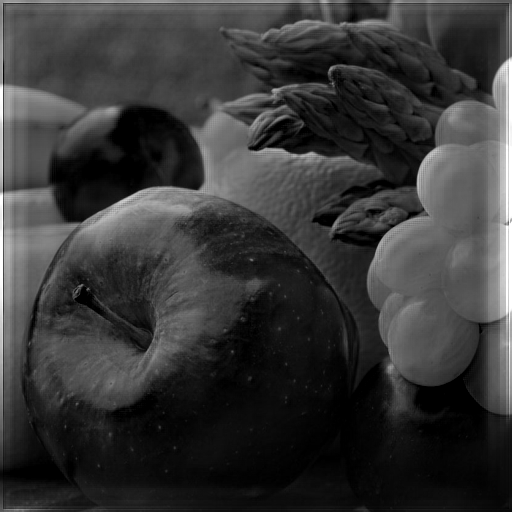
\includegraphics[width = 0.5\textwidth]{frutas_recons.png}  
  \caption{Reconstrucción de la imagen de frutas a partir de la pirámide de Laplace de 3 niveles.}
  \label{fig:frutasRec}
\end{figure}

\vspace{7cm}
\hrulefill
\par En la siguiente sección, se encuentra la implementación de todo lo descrito.  Por cada ítem, se muestra el código, explicación breve donde sea necesario y una prueba de la función implementada o el resultado que arroja esta. 
 
% \bigskip  
% \par Describir operación de convolución
% \par Describir brevemente cálculo de la pirámide de Gauss
% \par Describir brevemente cálculo de la pirámide de Laplace
% \par Describir brevemente reconstrucción de la imagen original


\newpage
\section{Desarrollo}
\subsection{Pirámide de \textit{Gauss}}

\subsubsection{Convolución}
\par A continuación, se presenta el código de la implementación de la convolución en \textit{Cython}:

\begin{lstlisting}[language=Python, label = convCode, caption=Implementación de convolución en Cython.]
  cpdef float[:, :] convolution_cython(float [:, :] input, float [:, :] mask):
  cdef int a, b, r, c, rows, cols, row_init, col_init, i, j,
  cdef float sum
  # Imagen de salida
  cdef np.ndarray output=np.zeros([input.shape[0], input.shape[1]], dtype = np.float32)

  # Posicion a partir de la cual se puede realizar convolucion: 
  # Ejemplo 1: Para un kernel de 3x3, es (1,1).
  # Ejemplo 2: Para un kernel de "a" x "b" es ("r"//2, "c"//2)
  a = mask.shape[0]
  b = mask.shape[1]

  row_init = a // 2
  col_init = b // 2

  # tamano de la imagen
  rows = input.shape[0]
  cols = input.shape[1]

  sum = 0

  # Recorremos la imagen input:
  for r in range(row_init, rows - row_init):
    for c in range(col_init, cols - col_init):
      # Se recorre la mascara o kernel:
      for i in range(a):
        for j in range(b):
          sum += mask[i,j] * input[r-i,c-j]
      # Guardamos el resultado de la suma correspondiente en el arreglo output:
      output[r, c] = sum
      sum = 0
  return output
\end{lstlisting}

\par La implementación en \ref{convCode}, corresponde a la convolución en dos dimensiones con padding. En el código, la sección más importante corresponde a los 4 ciclos de iteraciones anidados. Estos son los que recorren en primer lugar la imagen (\texttt{for r in rows} y luego \texttt{for c in columns}) y luego el \textit{kernel} guardando en la variable \texttt{sum} el resultado de operar para cada pixel \texttt{(r,c)} de la imagen, el resultado de la operación convolución. 


\par Para comparar la eficiencia de la función \texttt{convolution\_cython}, se comparó contra una implementada en el módulo \textit{scipy}. Para esto, se utilizó el comando \texttt{\%timeit}. Éste ejecuta una linea cierta cantidad de veces (100 en este caso) y guarda el mejor tiempo obtenido. Adicionalmente, utiliza distintos \textit{cores} para verificar que sea el mejor resultado: 

\begin{table}[H]
  \centering
  \begin{tabular}{|c|c|c|}
  \hline
                          & \textit{\textbf{Cython}} & \textit{\textbf{Scipy}} \\ \hline
  \textbf{Tiempo {[}ms{]}} & $15.8$                     & $3.08$                    \\ \hline
  \end{tabular}
  \caption{Tiempos de ejecución de operación convolución.}
  \label{profile}
\end{table}

\par Se observa en la tabla \ref{profile} que la función del módulo \textit{scipy} es varias veces mas rápida (puede variar cuánto más rápida es). De todas formas, se continuará utilizando la función implementada en \textit{cython}, siguiendo las instrucciones del enunciado.


\par A continuación se muestra un ejemplo de la ejecución de la función \texttt{convolution\_cython} con un \textit{kernel} de la siguiente forma (es un \textit{kernel} util para la detección de bordes):

\begin{equation}
\begin{bmatrix}
-1 & -1 & -1 \\ 
-1 & 8 & -1 \\ 
-1 & -1 & -1
\end{bmatrix}
\end{equation}

\begin{figure}[H]
  \centering
  \begin{subfigure}[t]{0.45\textwidth}
    \centering
    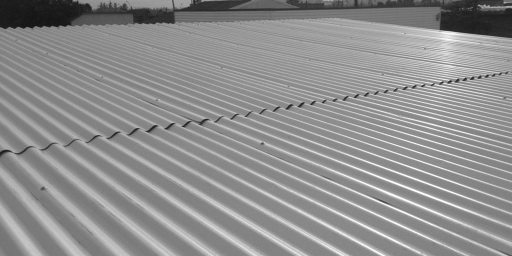
\includegraphics[width = 0.9\textwidth]{techo.png}
    \caption{Imagen original.}
  \end{subfigure}
  ~ 
  \begin{subfigure}[t]{0.45\textwidth}
      \centering
      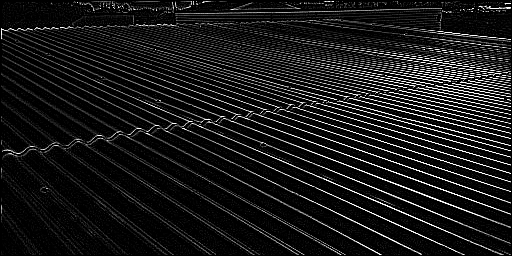
\includegraphics[width = 0.9\textwidth]{conv/techoconv.png}
      \caption{Imagen obtenida.}
  \end{subfigure}
  \caption{Salida obtenida al usar la función \textit{convolution\_cython}.}
  \label{convcython}
\end{figure}

\subsubsection{Cálculo de máscaras}

\begin{lstlisting}[language=Python, label = maskCode, caption=Cálculo de las máscaras en Python.]
def compute_gauss_horiz(sigma, width):
	mask = np.zeros([1, width], np.float32)

	
	coef = 1 / (sigma * np.sqrt(2 * np.pi))
 
	for i in range(width):
		mask[0][i] = coef * np.exp(- np.square(i - width//2) / (2 * sigma*sigma) )
		# Para debuggear
		#print((i - width//2))
	
	# normalizamos
  return mask / mask.sum()
  
def compute_gauss_vert(sigma, height):
	mask = np.zeros((height, 1), np.float32)
	# no es necesario implementar nuevamente la exponencial, solo trasponer el resultado
	# de la funcion comute_gauss_horiz
	hor_mask = compute_gauss_horiz(sigma = sigma, width = height)
	for i in range(height):
		mask[i][0] = hor_mask[0][i]
	return mask
\end{lstlisting}

\par Para el cálculo de los coeficientes del \textit{kernel}, se utilizó la siguiente ecuación:

\begin{equation}
  G(x,\sigma) \: = \: \frac{1}{\sigma \sqrt{2 \: \pi}} \exp(\tfrac{-x^2}{2 \sigma^2})
  \label{eqn:distGauss}
\end{equation}

\par Para que el cálculo sea correcto, se debe hacer un cambio de variable. Si el kernel es de una dimensión y de largo $n$, es de la forma:

\begin{equation}
  g(x) \: = \: [g_0,\: g_1,\:g_x,\: ...,\: g_n] , \: \: \: \: \: \:  \forall x \: \in \: [0,n]
\end{equation}

Pero la ecuación \ref{eqn:distGauss}, toma cada valor de $x$ con el centro del \textit{kernel} como referencia. Para resolver esto, en el código se hace el siguiente cambio de variables:

\begin{equation}
  x \: = \: i \: - \: n//2
\end{equation}

De esta forma, al recorrer desde $[0,n]$, se obtiene el valor correcto. El último paso para obtener el kernel es normalizar. A continuación, se muestra el resultado obtenido del cálculo de una máscara de una dimensión con $\sigma \: = \: 1$ y largo 3:


\begin{equation*}
  mask_{horizontal} \: = \: [[\: 0.27406862 ,\: 0.45186278 ,\: 0.27406862 \:]]
\end{equation*}

\par Para el cálculo de la máscara vertical, se obtiene una máscara horizontal y se transpone. El resultado entregado por la función \textit{compute\_gauss\_vert} con los mismos parámetros anteriores son:

\begin{equation*}
  mask_{vertical} \: = \: [[0.27406862],\: [0.45186278],\: [0.27406862]]
\end{equation*}

\subsubsection{Suavizado de imágenes}
\begin{lstlisting}[language=Python, label = blurCode, caption=Suavizado de imágenes.]
def do_blur(input, sigma, height):
	# Obtenemos las mascaras:
	hor_mask = compute_gauss_horiz(sigma, height)
	vert_mask = compute_gauss_vert(sigma, height)
	# Convolucion entre la imagen de entrada "input" y la mascara horizontal
	output = np.float32(convolution_cython(input, hor_mask))

	# Calcular convolucion entre la imagen resultante y la mascara vertical
	result = np.float32(convolution_cython(output, vert_mask) )

	return result
\end{lstlisting}

\par El suavizado de imágenes consiste en concatenar filtros: primero se aplica el filtro horizontal y luego el vertical. De esta forma se obtiene el suavizado (o \textit{blur}), que corresponde a un filtro pasabajo. 

\par En la figura \ref{blurtecho}, se muestra el resultado de aplicar \textit{blur} a la imagen del techo:

\begin{figure}[H]
  \centering
  \begin{subfigure}[t]{0.45\textwidth}
    \centering
    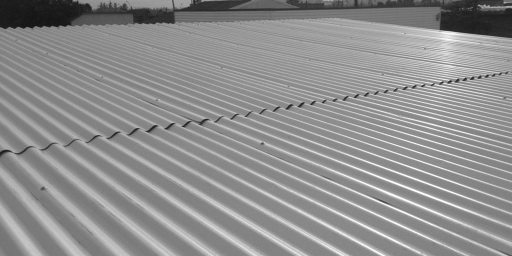
\includegraphics[width = 0.9\textwidth]{techo.png}
    \caption{Imagen original.}
  \end{subfigure}
  ~ 
  \begin{subfigure}[t]{0.45\textwidth}
      \centering
      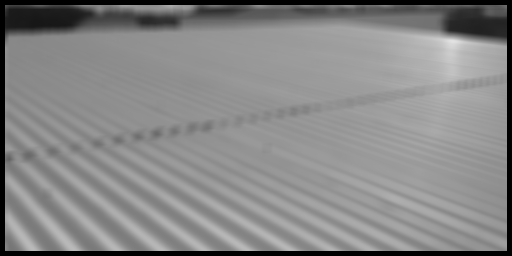
\includegraphics[width = 0.9\textwidth]{conv/techoblur.png}
      \caption{Imagen obtenida.}
  \end{subfigure}
  \caption{Salida obtenida al usar la función \textit{do\_blur}.}
  \label{blurtecho}
\end{figure}

\subsubsection{Submuestreo de la imagen}
\begin{lstlisting}[language=Python, label = subsampleCode, caption=Submuestreo de imágenes.]
def subsample(input):
  # Creamos el output. Tiene la mitad del ancho y del largo de la imagen original. 
	result = np.zeros(shape = [input.shape[0] // 2, input.shape[1] // 2], dtype = np.float32)
  
  # Nos quedamos con todos los pixeles pares (y el 0,0).
	for i in range(result.shape[0]):
		for j in range(result.shape[1]):
			result[i][j] = input[i*2][j*2]
			
	return result
\end{lstlisting}

\par Para el submuestreo, se solicitó que se guardaran sólo las columnas y las filas pares. Esto se asegura al recorrer la imagen original con el índice de la imagen de salida multiplicado por dos:

\begin{equation*}
  Output[i, j] \: = \: Input[2i, \: 2j],
\end{equation*}

Esto para los $i$ y $j$ mientras sean menores que $alto/2$ y $largo/2$. En la siguiente figura, se observa el resultado de aplicar el submuestreo a una imagen:

\begin{figure}[H]
  \centering
  \begin{subfigure}[t]{0.45\textwidth}
    \centering
    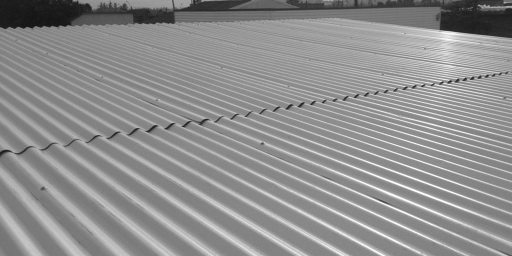
\includegraphics[width = 0.9\textwidth]{techo.png}
    \caption{Imagen original.}
  \end{subfigure}
  ~ 
  \begin{subfigure}[t]{0.45\textwidth}
      \centering
      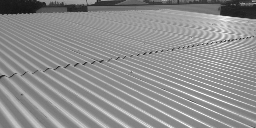
\includegraphics[width = 0.45\textwidth]{conv/techosub.png}
      \caption{Imagen obtenida.}
  \end{subfigure}
  \caption{Salida obtenida al usar la función \textit{subsample}.}
  \label{substecho}
\end{figure}

\par Es importante destacar que no solamente se escaló la imagen en el documento, sino que, al comprobar las dimensiones de cada una en Python, se obtiene el resultado esperado:

\begin{lstlisting}[language=Python, label = subsampletestCode, caption=Prueba del suavizado de imágenes.]
# Prueba de la funcion subsample
im_reduced = subsample(input)
print("entrada.shape = ", input.shape)
print("Salida.shape = ", im_reduced.shape)
# -----------Output generado en python-------------------
entrada.shape =  (256, 512)
Salida.shape =  (128, 256)
\end{lstlisting}


\subsubsection{Piramide de Gauss: computo y grafico}

\begin{lstlisting}[language=Python, label = gpCode, caption=Implementación pirámide de Gauss.]
# Calculo de la piramide de gauss:
def compute_gauss_pyramid(input, nlevels):  
  gausspyramid = []
  current = np.copy(input)
  gausspyramid.append(current)
  for i in range(1,nlevels):
    current = subsample(do_blur(input = gausspyramid[i-1], sigma = 2, height = 7))
    gausspyramid.append(current)
  return gausspyramid

# Display de la piramide de Gauss:
def show_gauss_pyramid(pyramid):
  for i, im in enumerate(pyramid):
    lvl = i + 1
    print("Imagen para nivel ", lvl)
    cv2_imshow( im )
\end{lstlisting}

\par La implementación de la pirámide de Gauss es simplemente concatenar lo realizado antes e iterar la cantidad de niveles que se deseen. De esta forma, en el primer nivel está la imagen original y en los siguentes se realiza lo siguente:

\begin{enumerate}
  \item Suavizar imagen del nivel anterior. 
  \item Submuestrear imagen obtenida en 1. 
  \item Agregar el resultado a la pirámide.
\end{enumerate}

\par Para graficar la pirámide de Gauss, solo se iteró sobre cada imagen que esta contiene y se utilizó la función \texttt{cv2\_imshow}.

\subsubsection{Resultados pirámide de Gauss}
\par En la siguiente sección, se muestran los resultados de aplicar lo anterior con los parámetros solicitados: 
\par \textbf{Frutas:}

\begin{figure}[H]
  \centering
  \begin{subfigure}[t]{0.48\textwidth}
    \centering
    \includegraphics[width = 0.9\textwidth]{frutas/gp1.png}
    \caption{Nivel 1.}
  \end{subfigure}
  ~ 
  \begin{subfigure}[t]{0.48\textwidth}
      \centering
      \includegraphics[width = 0.45\textwidth]{frutas/gp2.png}
      \caption{Nivel 2.}
  \end{subfigure}
  ~ 
  \begin{subfigure}[t]{0.32\textwidth}
      \centering
      \includegraphics[width = 0.45\textwidth]{frutas/gp3.png}
      \caption{Nivel 3.}
  \end{subfigure}
  ~ 
  \begin{subfigure}[t]{0.32\textwidth}
      \centering
      
\includegraphics[width = 0.22\textwidth]{frutas/gp4.png}
      \caption{Nivel 4.}
  \end{subfigure}
  ~ 
  \begin{subfigure}[t]{0.32\textwidth}
      \centering
      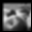
\includegraphics[width = 0.11\textwidth]{frutas/gp5.png}
      \caption{Nivel 5.}
  \end{subfigure}
  \caption{Pirámide de Gauss de la imagen \texttt{frutas.png}.}
  \label{gpfrutas}
\end{figure}

\par \textbf{Madera:}

\begin{figure}[H]
  \centering
  \begin{subfigure}[t]{0.48\textwidth}
    \centering
    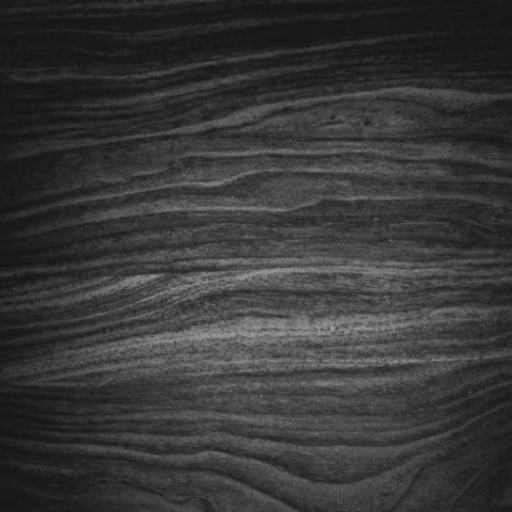
\includegraphics[width = 0.9\textwidth]{madera/gp1.png}
    \caption{Nivel 1.}
  \end{subfigure}
  ~ 
  \begin{subfigure}[t]{0.48\textwidth}
      \centering
      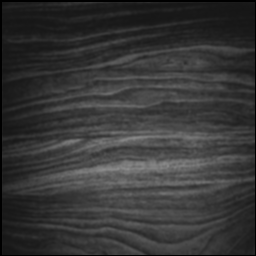
\includegraphics[width = 0.45\textwidth]{madera/gp2.png}
      \caption{Nivel 2.}
  \end{subfigure}
  ~ 
  \begin{subfigure}[t]{0.32\textwidth}
      \centering
      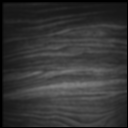
\includegraphics[width = 0.45\textwidth]{madera/gp3.png}
      \caption{Nivel 3.}
  \end{subfigure}
  ~ 
  \begin{subfigure}[t]{0.32\textwidth}
      \centering
      
\includegraphics[width = 0.22\textwidth]{madera/gp4.png}
      \caption{Nivel 4.}
  \end{subfigure}
  ~ 
  \begin{subfigure}[t]{0.32\textwidth}
      \centering
      
\includegraphics[width = 0.11\textwidth]{madera/gp5.png}
      \caption{Nivel 5.}
  \end{subfigure}
  \caption{Pirámide de Gauss de la imagen \texttt{madera.png}.}
  \label{gpmadera}
\end{figure}

\par \textbf{Poligonos:}

\begin{figure}[H]
  \centering
  \begin{subfigure}[t]{0.48\textwidth}
    \centering
    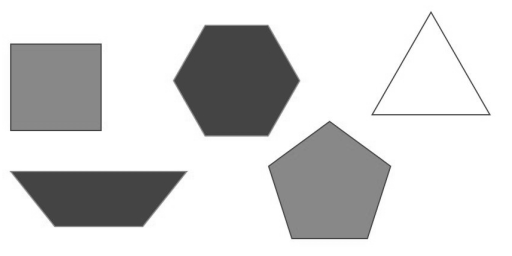
\includegraphics[width = 0.9\textwidth]{poligono/gp1.png}
    \caption{Nivel 1.}
  \end{subfigure}
  ~ 
  \begin{subfigure}[t]{0.48\textwidth}
      \centering
      
\includegraphics[width = 0.45\textwidth]{poligono/gp2.png}
      \caption{Nivel 2.}
  \end{subfigure}
  ~ 
  \begin{subfigure}[t]{0.32\textwidth}
      \centering
      
\includegraphics[width = 0.45\textwidth]{poligono/gp3.png}
      \caption{Nivel 3.}
  \end{subfigure}
  ~ 
  \begin{subfigure}[t]{0.32\textwidth}
      \centering
      
\includegraphics[width = 0.22\textwidth]{poligono/gp4.png}
      \caption{Nivel 4.}
  \end{subfigure}
  ~ 
  \begin{subfigure}[t]{0.32\textwidth}
      \centering
      
\includegraphics[width = 0.11\textwidth]{poligono/gp5.png}
      \caption{Nivel 5.}
  \end{subfigure}
  \caption{Pirámide de Gauss de la imagen \texttt{poligono.png}.}
  \label{gppoligono}
\end{figure}

\par \textbf{Techo:}

\begin{figure}[H]
  \centering
  \begin{subfigure}[t]{0.48\textwidth}
    \centering
    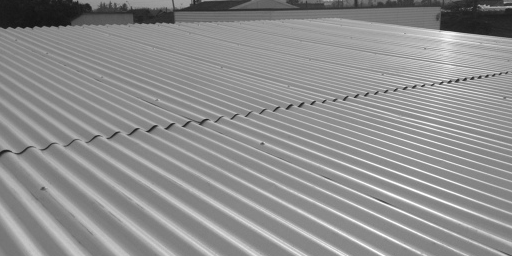
\includegraphics[width = 0.9\textwidth]{techo/gp1.png}
    \caption{Nivel 1.}
  \end{subfigure}
  ~ 
  \begin{subfigure}[t]{0.48\textwidth}
      \centering
      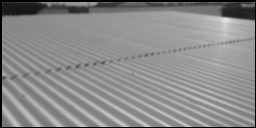
\includegraphics[width = 0.45\textwidth]{techo/gp2.png}
      \caption{Nivel 2.}
  \end{subfigure}
  ~ 
  \begin{subfigure}[t]{0.32\textwidth}
      \centering
      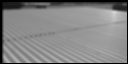
\includegraphics[width = 0.45\textwidth]{techo/gp3.png}
      \caption{Nivel 3.}
  \end{subfigure}
  ~ 
  \begin{subfigure}[t]{0.32\textwidth}
      \centering
      
\includegraphics[width = 0.22\textwidth]{techo/gp4.png}
      \caption{Nivel 4.}
  \end{subfigure}
  ~ 
  \begin{subfigure}[t]{0.32\textwidth}
      \centering
      
\includegraphics[width = 0.11\textwidth]{techo/gp5.png}
      \caption{Nivel 5.}
  \end{subfigure}
  \caption{Pirámide de Gauss de la imagen \texttt{techo.png}.}
  \label{gptecho}
\end{figure}

\subsection{Analisis pirámide de Gauss}
En primer lugar, es importante destacar que el resultado obtenido en la pirámide de Gauss depende de varios parámetros: 

\begin{itemize}
  \item \textbf{Niveles:} Cantidad de niveles que tendrá la pirámide. 
  \item \textbf{$\sigma$:} Desviación estándar para el filtro \textit{blur}.
  \item \textbf{\textit{Height}:} Tamaño del filtro \textit{blur}.
\end{itemize}

Por otro lado, se observa que los resultados son similares independiente de la imagen: En todos los casos, se observa la evidente reducción del tamaño (recordar que además estan escaladas en el documento, de otra forma se los ultimos niveles no se distinguían) y se observa también el efecto del filtro \textit{blur}. El principal efecto es que los bordes se suavizan. Se notó también que a mayor $\sigma$ o \textit{Height}, este efecto se notaba más en las imágenes de salida. 


%- Describir implementación de convolución, incluyendo código
%- Describir implementación de cálculo de máscaras, incluyendo código
% - Describir implementación de suavizado de imágenes, incluyendo código
% - Describir implementación de submuestreo, incluyendo código
% - Describir implementación de pirámide de Gauss, incluyendo código
% - Describir implementación: graficar pirámide de Gauss, incluyendo código
% - Prueba del sistema de cálculo de pirámide de Gauss sobre 4 imágenes entregadas, incluir las
% imágenes de las pirámides resultantes en el informe
% - Análisis del desempeño del cálculo de la pirámide de Gauss, analizando las imágenes resultantes


\newpage
\subsection{Pirámide de \textit{Laplace}}
\subsubsection{Resta de imágenes}

\begin{lstlisting}[language=Python, label = subCode, caption=Implementación resta de imágenes.]
def subtract(input1, input2):
  # Verificamos que sean del mismo tamano
  assert (input1.shape == input2.shape), "Imagenes deben tener igual tamano"
  
  output = input1 - input2
  return output
\end{lstlisting}

\par Para la función \textit{subtract}, se debe verificar en primer lugar que ambas imágenes tengan igual dimensión. En caso de no ser así arroja error. Luego, simplemente se resta una imagen con la otra. 


\subsubsection{Pirámide de Laplace}
\begin{lstlisting}[language=Python, label = lpCode, caption=Cómputo pirámide de Laplace.]
def compute_laplace_pyramid(input, nlevels):
  gausspyramid = []
  laplacepyramid = []
  current = np.copy(input)
  gausspyramid.append(current)
  for i in range(1, nlevels):
    # Por hacer:
    # 1) Aplicar do_blur( ) a la imagen gausspyramid[i-1], con sigma 2.0 y ancho 7
    blur_im = do_blur(input = gausspyramid[i-1], sigma = 2, height = 7)
    # 2) Guardar en laplacepiramid el resultado de restar gausspyramid[i - 1] y la imagen calculada en (1)
    laplacepyramid.append(np.float32(subtract(input1 = gausspyramid[i-1], input2 = blur_im)))
    # 3) Submuestrear la imagen calculada en (1), guardar el resultado en current
    current = subsample( input = blur_im )
    gausspyramid.append(current)
  laplacepyramid.append(current)  # Se agrega el ultimo piso de la piramide de Laplace
  return laplacepyramid
\end{lstlisting}

\par El cálculo de la pirámide de Laplace, como se mencionó en la sección \ref{lpsection}, consiste en almacenar la información perdida entre un nivel y otro de la pirámide de Gauss. Para esto, se comienza con el primer piso de la pirámide de Gauss y luego se itera en lo siguiente (paso $i$ de la iteración):

\begin{enumerate}
  \item Suavizar (filtro \textit{blur}) imagen del piso anterior de la pirámide de gauss ($GaussPiramyd[i-1]$). 
  \item Restar la imagen obtenida con la original ($GaussPiramyd[i-1]$ menos imagen recién obtenida).
  \item Agregar lo obtenido a la pirámide de Laplace. 
\end{enumerate}

\subsubsection{Escalamiento y valor absoluto de la imágen}
\begin{lstlisting}[language=Python, label = scaleabsCode, caption=Función \textit{scale\_abs}.]
def scale_abs(input, factor):
  # Creamos imagen de salida del mismo tamano del de la entrada
  output = np.zeros_like(input)
  # Por hacer: aplicar valor absoluto a los pixeles de la imagen pixel a pixel y luego escalar los pixeles usando el factor indicado
  for i in range(input.shape[0]):
    for j in range(input.shape[1]):
      output[i][j] = np.abs(input[i][j]) * factor
  
  return np.float32(output)
\end{lstlisting}

\par En la implementación se observa que lo que se hace es simplemente iterar por todos los pixeles calculando el valor absoluto y luego escalando por un factor ($factor$) que es un \textit{input} de la función. 

\subsubsection{Graficar pirámide de Laplace}
\begin{lstlisting}[language=Python, label = showlpCode, caption=Función para graficar pirámide de Laplace.]
def show_laplace_pyramid(pyramid):
  # Por hacer: mostrar las imagenes de la piramide de laplace:
  #  Las imagenes deben ser escaladas antes de mostrarse usando scale_abs
  #  Sin embargo, la ultima imagen del ultimo piso se muestra tal cual
  # Se recomienda usar cv2_imshow( ) para mostrar las imagenes
  for i, im in enumerate(pyramid):
    lvl = i + 1
    print("Imagen para nivel ", lvl)
    # Se escalan todas menos la ultima
    if i != len(pyramid)-1:
      cv2_imshow( scale_abs(im, 5) )
    else:
      cv2_imshow( im ) 
\end{lstlisting}

\par En esta función cada imagen, excepto la última, debe ser escalada antes de mostrarse. Para esto, se agrega el \texttt{if} en la línea 10. 

\subsubsection{Resultados pirámide de Laplace}
A continuación, se muestran los resultados obtenidos de aplicar el cálculo de las pirámides de Laplace a las 4 imágenes con los parámetros solicitados:

\par \textbf{Frutas:}

\begin{figure}[H]
  \centering
  \begin{subfigure}[t]{0.48\textwidth}
    \centering
    \includegraphics[width = 0.9\textwidth]{frutas/lp1.png}
    \caption{Nivel 1.}
  \end{subfigure}
  ~ 
  \begin{subfigure}[t]{0.48\textwidth}
      \centering
      \includegraphics[width = 0.45\textwidth]{frutas/lp2.png}
      \caption{Nivel 2.}
  \end{subfigure}
  ~ 
  \begin{subfigure}[t]{0.32\textwidth}
      \centering
      
\includegraphics[width = 0.45\textwidth]{frutas/lp3.png}
      \caption{Nivel 3.}
  \end{subfigure}
  ~ 
  \begin{subfigure}[t]{0.32\textwidth}
      \centering
      
\includegraphics[width = 0.22\textwidth]{frutas/lp4.png}
      \caption{Nivel 4.}
  \end{subfigure}
  ~ 
  \begin{subfigure}[t]{0.32\textwidth}
      \centering
      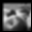
\includegraphics[width = 0.11\textwidth]{frutas/lp5.png}
      \caption{Nivel 5.}
  \end{subfigure}
  \caption{Pirámide de Laplace de la imagen \texttt{frutas.png}.}
  \label{lpfrutas}
\end{figure}

\par \textbf{Madera:}

\begin{figure}[H]
  \centering
  \begin{subfigure}[t]{0.48\textwidth}
    \centering
    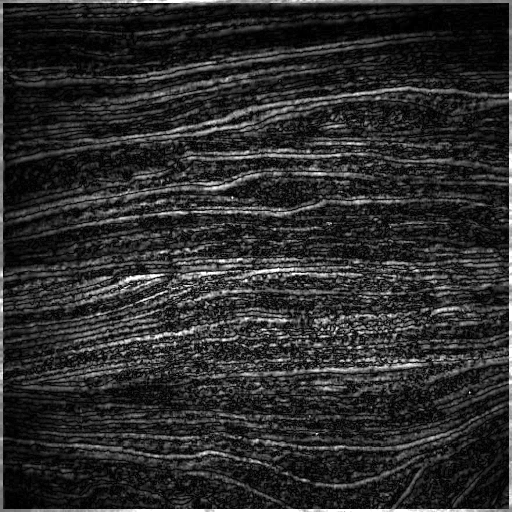
\includegraphics[width = 0.9\textwidth]{madera/lp1.png}
    \caption{Nivel 1.}
  \end{subfigure}
  ~ 
  \begin{subfigure}[t]{0.48\textwidth}
      \centering
      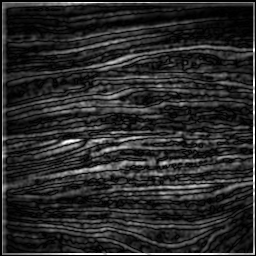
\includegraphics[width = 0.45\textwidth]{madera/lp2.png}
      \caption{Nivel 2.}
  \end{subfigure}
  ~ 
  \begin{subfigure}[t]{0.32\textwidth}
      \centering
      
\includegraphics[width = 0.45\textwidth]{madera/lp3.png}
      \caption{Nivel 3.}
  \end{subfigure}
  ~ 
  \begin{subfigure}[t]{0.32\textwidth}
      \centering
      
\includegraphics[width = 0.22\textwidth]{madera/lp4.png}
      \caption{Nivel 4.}
  \end{subfigure}
  ~ 
  \begin{subfigure}[t]{0.32\textwidth}
      \centering
      
\includegraphics[width = 0.11\textwidth]{madera/lp5.png}
      \caption{Nivel 5.}
  \end{subfigure}
  \caption{Pirámide de Laplace de la imagen \texttt{madera.png}.}
  \label{lpmadera}
\end{figure}

\par \textbf{Poligonos:}

\begin{figure}[H]
  \centering
  \begin{subfigure}[t]{0.48\textwidth}
    \centering
    \includegraphics[width = 0.9\textwidth]{poligono/lp1.png}
    \caption{Nivel 1.}
  \end{subfigure}
  ~ 
  \begin{subfigure}[t]{0.48\textwidth}
      \centering
      \includegraphics[width = 0.45\textwidth]{poligono/lp2.png}
      \caption{Nivel 2.}
  \end{subfigure}
  ~ 
  \begin{subfigure}[t]{0.32\textwidth}
      \centering
      \includegraphics[width = 0.45\textwidth]{poligono/lp3.png}
      \caption{Nivel 3.}
  \end{subfigure}
  ~ 
  \begin{subfigure}[t]{0.32\textwidth}
      \centering
      \includegraphics[width = 0.22\textwidth]{poligono/lp4.png}
      \caption{Nivel 4.}
  \end{subfigure}
  ~ 
  \begin{subfigure}[t]{0.32\textwidth}
      \centering
      \includegraphics[width = 0.11\textwidth]{poligono/lp5.png}
      \caption{Nivel 5.}
  \end{subfigure}
  \caption{Pirámide de Laplace de la imagen \texttt{poligono.png}.}
  \label{lppoligono}
\end{figure}

\par \textbf{Techo:}

\begin{figure}[H]
  \centering
  \begin{subfigure}[t]{0.48\textwidth}
    \centering
    \includegraphics[width = 0.9\textwidth]{techo/lp1.png}
    \caption{Nivel 1.}
  \end{subfigure}
  ~ 
  \begin{subfigure}[t]{0.48\textwidth}
      \centering
      \includegraphics[width = 0.45\textwidth]{techo/lp2.png}
      \caption{Nivel 2.}
  \end{subfigure}
  ~ 
  \begin{subfigure}[t]{0.32\textwidth}
      \centering
      \includegraphics[width = 0.45\textwidth]{techo/lp3.png}
      \caption{Nivel 3.}
  \end{subfigure}
  ~ 
  \begin{subfigure}[t]{0.32\textwidth}
      \centering
      \includegraphics[width = 0.22\textwidth]{techo/lp4.png}
      \caption{Nivel 4.}
  \end{subfigure}
  ~ 
  \begin{subfigure}[t]{0.32\textwidth}
      \centering
      \includegraphics[width = 0.11\textwidth]{techo/lp5.png}
      \caption{Nivel 5.}
  \end{subfigure}
  \caption{Pirámide de Laplace de la imagen \texttt{techo.png}.}
  \label{lptecho}
\end{figure}


\subsection{Analisis pirámide de Laplace}
A diferencia de la pirámide de Gauss, en este caso la imagen de entrada afecta notablemente los resultados obtenidos. Esto se nota claramente en particular en la figura \ref{lppoligono}. Se observa que los bordes detectados, a medida que se aumenta el nivel de la pirámide, se observa de peor forma. 

\par Se observa además que, debido al \textit{padding} realizado en la convolución y a que esta pirámide es un filtro para detección de bordes (entre otros),  los resultados se ven más afectados que en la pirámide de Gauss. 

\par Es importante destacar que, dentro de las aplicaciones de las pirámides, ésta es en particular útil porque permite comprimir el espacio que ocupa una imagen en memoria. Esto no es evidente debido a que a partir de una imagen se generan 5. Pero es fácil observar también que gran parte de los bits o píxeles serán cercanos a cero. Por esto, puede resultar más compacto en temas de memoria para almacenar una imagen. \cite{paperPyramids}

% - Describir implementación de resta de imágenes, incluyendo código
% - Describir implementación de pirámide de Laplace, incluyendo código
% - Describir implementación de valor absoluto y escalamiento, incluyendo código
% - Describir implementación: graficar pirámide de Laplace, incluyendo código
% - Prueba del sistema de cálculo de pirámide de Laplace sobre 4 imágenes entregadas, incluir las
% imágenes de las pirámides resultantes en el informe
% - Análisis del desempeño del cálculo de la pirámide de Laplace, analizando las imágenes resultantes


\subsection{Reconstrucción imagen}
\subsubsection{Suma de imágenes}
\begin{lstlisting}[language=Python, label = addCode, caption=Función suma de imágenes.]
def add(input1, input2):
  # Verificamos que sean del mismo tamano
  assert (input1.shape == input2.shape), "Imagenes deben tener igual tamano"
  output = input1 + input2
  return output
\end{lstlisting}

\par Para la función \textit{add}, se debe verificar en primer lugar que ambas imágenes tengan igual dimensión. En caso de no ser así arroja error. Luego, simplemente se suma una imagen con la otra. 

\subsubsection{\textit{Upsample}: Duplicado del tamaño de la imagen}
\begin{lstlisting}[language=Python, label = upsampleCode, caption=Función \textit{upsample}.]
def upsample(input):
  # Por hacer: implementar duplicacion del tamano de imagen pixel a pixel
  # Un pixel de la imagen de salida debe ser el promedio de los 4 pixeles mas cercanos de la imagen de entrada

  def get_neighbours(input,i,j):
    ''' FUNCION AUXILIAR
    Funcion que entrega el promedio de los 4 pixeles mas cercanos.
    Args: 
      input: imagen de entrada
    '''
    counter = 0
    # Se realizan 4 bloques de try/except para que al llegar a los bordes, no arroje
    #errores la funcion. 
    try:
      a = input[i][j-1]
      counter += 1
    except IndexError:
      a = 0
    
    try:
      b = input[i][j+1]
      counter += 1
    except IndexError:
      b = 0

    try:
      c = input[i-1][j]
      counter += 1
    except IndexError:
      c = 0
    
    try:
      c = input[i-1][j]
      counter += 1
    except IndexError:
      c = 0

    try:
      d = input[i+1][j]
      counter += 1
    except IndexError:
      d = 0

    result = (input[i][j] + a + b + c + d)/(counter + 1)
    
    return np.float32(result)

  # Se debe tener cuidado de que los indices no salgan fuera del tamano de la imagen
  output = np.zeros(shape = [input.shape[0]*2, input.shape[1]*2], dtype = np.float32)
  for i in range(output.shape[0]):
    for j in range(output.shape[1]):
      output[i][j] = get_neighbours(input,i//2, j//2)
  return output
\end{lstlisting}

\par Para la implementación de la función \textit{upsample}, se debía recorrer la imagen original de la siguiente forma:

\begin{gather}
  \begin{aligned}
      output[i,j] \: = \: \tfrac{1}{coef} ( \: input[i//2,\: j//2] & \: + \: input[i//2,\:\: j//2-1] \\  
                                          & \: + \: input[i//2-1,\:\: j//2] \\  
                                          & \: + \: input[i//2,\:\: j//2+1] \\   
                                          & \: + \: input[i//2+1,\:\: j//2] \: )
  \end{aligned}
\end{gather}

Donde $coef$ se utiliza para calcular el promedio y corresponde a la cantidad de $input$ que efectivamente existen. Esto porque en los bordes de la imagen puede no existir el elemento $[i//2,j//2 +1]$, por ejemplo.

\par De esta forma, se obtiene para cada pixel, el primedio de sus vecinos (y el mismo) y se agrega a la immagen de salida. 

\par Para manejar los errores que puedan ocurrir al intentar obtener los vecinos de cada pixel, se implementó una función auxiliar llamada \textit{get\_neighbours}. Ésta se encarga de resolver los problemas de los casos bordes con bloques \texttt{try, except} y entrega el promedio de los 4 vecinos más cercanos al pixel $[i,j]$.

\subsubsection{Reconstrucción de imagen}
\begin{lstlisting}[language=Python, label = reconstrCode, caption=Función de reconstrucción de la imagen.]
def reconstruct(laplacepyramid):
  output = []
  lvls = len(laplacepyramid)
  output.append(laplacepyramid[lvls - 1])
  for i in range(lvls - 1):
    # Por hacer: repetir estos dos pasos:
    # (1) Duplicar tamano output usando upsample( )
    # (2) Sumar resultado de (1) y laplacepyramid[lev] usando add( ), almacenar en output
    output.append(add(input1 = upsample(output[i]), input2 = laplacepyramid[lvls -i -2]))
  return output[len(output) -1]
\end{lstlisting}


En la sección \ref{reconstimagensection}, se describe la iteración necesaria para reconstruir la imagen: 
\begin{enumerate}
  \item Duplicar el tamaño de la imagen.
  \item Sumar la imagen duplicada con el siguiente piso de la pirámide de Laplace. 
\end{enumerate}

En el código, estos dos pasos se hacen en una misma línea (línea 10), para luego seguir iterando. Es importante notar que se podría devolver una imagen reconstruída para cada nivel pero se devuelve sólo la final. 


\subsection{Resultados reconstrucción}
A continuación, se muestran los resultados de la reconstrucción de las 4 imágenes:

\begin{figure}[H]
  \centering
  \begin{subfigure}[t]{0.46\textwidth}
    \centering
    \includegraphics[width = 0.9\textwidth]{frutas/reconstr.png}
    \caption{Frutas reconstruidas.}
  \end{subfigure}
  ~ 
  \begin{subfigure}[t]{0.46\textwidth}
      \centering
      \includegraphics[width = 0.9\textwidth]{madera/reconstr.png}
      \caption{Madera reconstruida.}
  \end{subfigure}
  ~ 
  \begin{subfigure}[t]{0.46\textwidth}
      \centering
      \includegraphics[width = 0.9\textwidth]{poligono/reconstr.png}
      \caption{Poligonos reconstruidos.}
  \end{subfigure}
  ~ 
  \begin{subfigure}[t]{0.46\textwidth}
      \centering
      \includegraphics[width = 0.9\textwidth]{techo/reconstr.png}
      \caption{Techo reconstruido.}
  \end{subfigure}
  \caption{Reconstrucción de las 4 imágenes.}
  \label{reconstrIm}
\end{figure}

\subsection{Análisis reconstrucción de imagen}

\par En primer lugar, se observan grandes diferencias en los resultados obtenidos en cada imagen independiente de la `complegidad' de cada imagen. Por ejemplo, una imagen que contiene solo 5 figuras geométricas obtiene peores resultados que la imagen de la madera. 

\par En particular, en la imagen de los polígonos, se observa además como los artefactos que se observan en la pirámide de Laplace (en la figura \ref{lppoligono}), se observan también en la reconstrucción de la imagen.

\par Se observa por otro lado, que el problema generado por la implementación de \textit{padding}, la reconstrucción en los bordes de la figura contiene artefactos: un marco que dependiendo de la cantidad de niveles de la pirámide, es cuanto cubre la imagen generada. 


\newpage
\section{Conclusión}
Se adquirió conociemiento sobre una nueva forma de hacer más eficiente el código en Python con \textit{Cython}. Esta permite escribir funciones, clases y otros, en bajo nivel y ahorrar tiempo de ejecución debido a las ventajas de \texttt{C} por sobre \texttt{Python}. Por ejemplo, asignación del tipo de variables (y no asignación dinámica como lo es python), y otras ventajas más. 

\par Al comparar la velocidad de la función \textit{convolution\_cython} con la implementada en el módulo \texttt{scipy.signal}, se observó que esta no era mejor. Por esto, se comprende el carácter pedagógico de implementar la convolución en \textit{cython}. El objetivo era comprender el costo computacional de estas operaciones y comprender como operan sobre las imágenes. 

\par Se observó el efecto de `inventar' información al realizar \textit{padding}. Este además fue la causa de que al reconstruir las imágenes se obtubieran resultados no excelentes. Esto se puede solucionar implementando otro tipo de \textit{padding}: rellenar en lugar de con ceros, con el promedio de los pixeles más cercanos. 

\par Durante la confección del informe, se aprendió sobre distintas utilidades de las piramides descritas en el paper \cite{paperPyramids}. Estas van desde generar distintas representaciones de una imagen u objeto para detección hasta compresión en memoria de las imágenes. 

\newpage
\begin{thebibliography}{X}
  \bibitem{imConv2d} Towards Data Science: Intuitively Understanding Convolutions for Deep Learning. By Irhum Shafkat. \\
  \url{https://towardsdatascience.com/intuitively-understanding-convolutions-for-deep-learning-1f6f42faee1}   

  \bibitem{WikiConv} Wikipedia: Convolution. \\
  \url{https://en.wikipedia.org/wiki/Convolution#Visual_explanation} 

  \bibitem{paperPyramids} Pyramid methods in image processing. E. H. Adelson, C. H. Anderson,  J. R. Bergen,  P. J. Burt,  J. M. Ogden. $[1984]$
  \url{http://persci.mit.edu/pub_pdfs/RCA84.pdf}

\end{thebibliography}

\section{Anexos}
\end{document}